% тут сейчас будут очевидные коментарии
\documentclass[12pt,a4paper]{scrbook} %{article}
\usepackage[utf8]{inputenc}				% кодировка утф8
\usepackage[T2A]{fontenc}
\usepackage[russian]{babel}				% локализация
\usepackage{misccorr}					% пакет с дополнительными настройками для соответствия правилам отечественной полиграфии (не знаю, нужен ли, тупо скопипастил)
\usepackage{color}
\usepackage{graphicx}			% чтоб картинки вставлять
\usepackage{amsmath}					% для формул
\usepackage{amsfonts}
\usepackage{amssymb}
\usepackage{listings}                   % для вставок кода
\usepackage{hyperref}                   % оформление ссылок
\usepackage{blindtext}

\graphicspath{ {pic} }       % путь до картинок




%\color[named]{BrickRed}
%\pagecolor[named]{Green}

\title{Построение собственного USB устройства ввода в Linux, имея только голый чип}
\subtitle{Version 1.0}
\author{Михаил Белкин}
\date{Август 2021}

\begin{document}
\maketitle
\tableofcontents

\section{Схемотехника.}
\subsection{Выбор редактора.}
    Разработка схемы производится в KiCAD, это очень легковесный и компактный
    opensource редактор. Но при этом несмотря на его внешнюю простоту редактор
    как будто бы кричит нам "Я ничем не хуже чем этот ваш Altium и уж тем более
    Eagle". Поддерживается редактирование многослойных плат, так же используется
    профессиональный подход, при котором схема устройства и печатная плата
    редактируются отдельно. Так же он очень нетребователен к ресурсам
    компьютера.

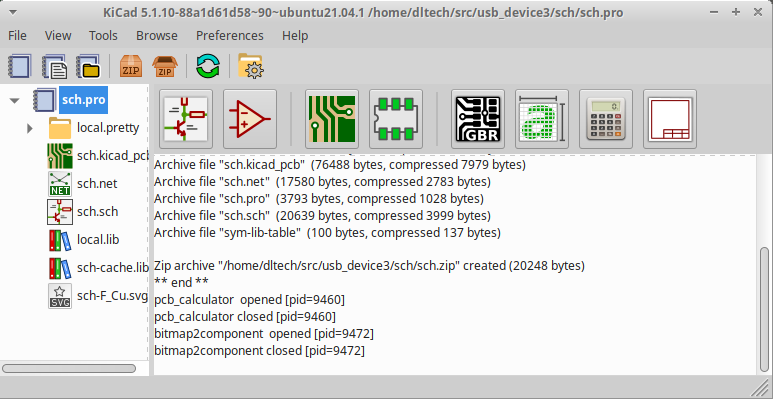
\includegraphics[width=10cm]{kicad1.png}

    К редактору имеется собственная библиотека компонентов, которая включает в
    себя компоненты всех популярных производителей. Но если вы принесли
    с китайского базара какую то экзотику, компонент придется разработать
    самостоятельно.\\
    Вывод шаблона печатной платы возможен во всех удобный форматах, включая pdf.
    Так же и Gerber и векторный svg, последнее очень удобно для печати шаблона
    на принтере. Единственное неудобство это не возможность сразу выводить схему
    в растровом формате, приходится самостоятельно конвертировать из svg.
\subsection{Установка редактора и библиотек.}
    Установка редактора в Ubuntu Linux производится очень просто, имеется
    отдельный ppa репозиторий с последней стабильной версией. В то время как
    наиболее полный набор библиотек компонентов можно скачать с гитхаба.\\
    Набор команд для установки KiCAD:
\lstset{language=bash}           % Задаем язык исходного кода
\begin{lstlisting}
sudo add-apt-repository --yes ppa:kicad/kicad-5.1-releases
sudo apt update
sudo apt install --install-recommends kicad
\end{lstlisting}

    Надеюсь устанавливать git вы умеете и про команду git clone вы тоже знаете.
    Вот ссылки на репозитории с библиотеками компонентов KiCAD:\\
    \url{https://github.com/KiCad/kicad-library}\\
    \url{https://github.com/KiCad/kicad-footprints}\\
    \url{https://github.com/KiCad/kicad-symbols}\\
    \url{https://github.com/KiCad/kicad-packages3D}\\

    При этом важно отметить, что устройство

\subsection{Выбор элементной базы.}
    Для наиболее аккуратной реализации нужен современный микроконтроллер с
    полноценным аппаратным USB. Совершенно понятно, что таким микроконтроллером
    окажетcя STM32F103C8T6. Мощное ядро ARM Cortex-M3 с их фирменным вложенным
    контроллером прерываний (NVIC) позволит с легкостью справиться с любой
    задачей. А с такой простой как USB геймпад уж тем более. На борту имеется
    64 килобайта FLASH и 20 килобайт SRAM. И этого настолько много, что можно
    вовсе не думать об оптимизации. Теперь о стоимости, когда то я покупал такой
    за 60 рублей, сейчас цена приблизилась к 200, что по прежнему сравнимо по
    стоимости с остальными морально устаревшими микроконтроллерами. Так же в
    пользу данного микроконтроллера говорит наличие подробной
    документации. О том, почему именно F103, тут все просто, это самый дешевый
    МК с USB из тех что может предложить компания ST microelectronics.
\subsection{Особенность схемотехники USB.}
\subsection{Схема устройства.}

\section{Программное обеспечение.}

    \subsection{Тулчейн.}
    \subsection{Базовые библиотеки для микроконтроллера.}
    \subsection{Структура моего ПО.}
    \subsection{Опрос кнопок.}
    \subsection{Периферия USB.}
    \subsection{Дескрипоры USB.}
    \subsection{Стандартный протокол USB.}
    \subsection{USB HID}
    \subsection{Отладка.}


	%\includegraphics[scale=1]{pictures/minicom.eps}

\begin{thebibliography}{9}

\bibitem{lamport94}
  Leslie Lamport,
  Addison Wesley, Massachusetts,
  2nd edition,
  1994.

\end{thebibliography}

\end{document}
